%
% Tesi D.S.I. - modello preso da
% Stanford University PhD thesis style -- modifications to the report style
%
%%%%%%%%%%%%%%%%%%%%%%%%%%%%%%%%%%%%%%%%%%%%%%%%%%%%%%%%%%%%%%%%%%%%%%%%%%%
%                                                                         %
%			TESI DOTTORATO                                                   %
%			______________                                                   %
%                                                                         %
%			AUTORE: Elena Pagani                                             %
%                                                                         %
%			Ultima revisione: 7.X.1998                                       %
%                                                                         %
%%%%%%%%%%%%%%%%%%%%%%%%%%%%%%%%%%%%%%%%%%%%%%%%%%%%%%%%%%%%%%%%%%%%%%%%%%%
%
%
\documentclass[12pt]{report}
%    \renewcommand{\baselinestretch}{1.6}      % interline spacing
%
% \includeonly{}
%
%			PREAMBOLO
%
\usepackage[a4paper]{geometry}
\usepackage{amssymb,amsmath,amsthm}
\usepackage{graphicx}
\usepackage{url}
\usepackage{hyperref}
\usepackage{epsfig}
\usepackage[italian]{babel}
\usepackage{tesi}
\usepackage{float}
% per le accentate
\usepackage[T1]{fontenc}
\usepackage[utf8]{inputenc}
\usepackage{hyperref}
%
\newtheorem{myteor}{Teorema}[section]
%
\newenvironment{teor}{\begin{myteor}\sl}{\end{myteor}}
%
%
%			TITOLO
%
\begin{document}
\begin{center}
	
\includegraphics[height=3.0cm]{logo_unimi.png}
\end{center}

\title{Sviluppare il pensiero computazionale con i quesiti Bebras: approcci e strumenti per l'uso nella pratica scolastica.}
\author{Annalisa CALCAGNI}
\dept{Corso di Laurea Magistrale in Informatica } 
\anno{2016-2017}
\matricola{865610}
\relatore{Prof. Violetta LONATI}
\correlatore{Prof. Mattia MONGA}
%
%        \submitdate{month year in which submitted to GPO}
%		- date LaTeX'd if omitted
%	\copyrightyear{year degree conferred (next year if submitted in Dec.)}
%		- year LaTeX'd (or next year, in December) if omitted
%	\copyrighttrue or \copyrightfalse
%		- produce or don't produce a copyright page (false by default)
%	\figurespagetrue or \figurespagefalse
%		- produce or don't produce a List of Figures page
%		  (false by default)
%	\tablespagetrue or \tablespagefalse
%		- produce or don't produce a List of Tables page
%		  (false by default)
% 
%			DEDICA
%
\beforepreface
        {\hfill \Large {\sl dedicato a \dots}}
% 
\afterpreface
%			PREFAZIONE: Introduzione
%
\prefacesection{Introduzione}
hkjafgyruet
%
%
%
% 
% 
%			CAPITOLO 1: Bebras
\chapter{Bebras}
\label{cap1}
%
\section{Bebras a livello mondiale}
Negli ultimi dieci anni in tutto il mondo sono state organizzate numerose gare riguardanti l'Informatica, principalmente per due motivi: selezionare studenti particolarmente talentuosi in questo campo, come accade nelle Olimpiadi Informatiche, oppure diffondere fin dalle prime fasi dell'educazione i concetti base di questa disciplina scientifica che spesso nelle scuole si finisce per confondere con le "applicazioni" dell'Informatica. Quest'ultimo è esattamente lo scopo del Bebras, il quale è una gara organizzata annualmente dal 2004 in più paesi (50 nel 2016), con un numero di partecipanti superiore a mezzo milione nelle ultime edizioni.\cite{BellettiniITICSE2015}
Bebras ("castoro" nella lingua del Paese, la Lituania, dove è nata l'iniziativa) è un'organizzazione internazionale che ha lo scopo di promuovere nelle scuole gli aspetti scientifici dell'informatica. I giochi Bebras sono accessibili agli studenti delle scuole primarie e secondarie anche senza nessuna specifica conoscenza pregressa. Gli studenti partecipano a questa gara attraverso il computer direttamente dalle proprie scuole, sotto la supervisione di un loro insegnante, il quale successivamente può integrare la correzione della suddetta gara all'interno delle attività curricolari.

La gara Bebras è composta da quesiti di due tipi: domande a scelta multipla con quattro risposte e problemi interattivi. Il numero di quesiti varia da un anno all'altro: da diciotto a ventiquattro domande di difficoltà diverse, da risolvere in 40, 45 o 55 minuti.
Il Bebras è organizzato annualmente a livello locale, dalla delegazione del Paese partecipante, la quale utilizza tecnologie diverse per l'esecuzione della gara, ma generalmente tutti usano sistemi di gestione online.
Ogni delegazione sceglie, da un insieme di quesiti approvati dalla comunità internazionale, quelli da inserire nella loro edizione locale del Bebras, ma alcuni di essi sono da utilizzare obbligatoriamente.
\newpage
I quesiti sono divisi in sei categorie:
\begin{itemize}
\item Pre-Primary: 5-8 anni
\item Primary: 8-10 anni
\item Benjamins: 10-12 anni
\item Cadets: 12-14 anni
\item Juniors: 14-16 anni
\item  Seniors: 16-19 anni
\end{itemize}
Ogni delegazione locale può riorganizzare le proprie categorie a seconda delle proprie realtà scolastiche.
\\

Il cuore dell'organizzazione di questa gara è un workshop annuale internazionale che riunisce delegati provenienti da tutti i Paesi coinvolti, con lo scopo di proporre e correggere i quesiti da sottoporre ai partecipanti.  
Ogni Paese partecipante è invitato a fornire almeno un mese prima del workshop un insieme di proposte di quesiti, che sono resi disponibili per essere visionati e commentati. Durante i tre giorni di lavoro, i partecipanti vengono divisi in gruppi ad ognuno dei quali viene assegnato un insieme di quesiti su cui discutere. Alla fine dei giorni di lavoro ogni gruppo proporrà una serie di quesiti candidati ad essere quelli obbligatori, ma diverranno tali solo dopo la votazione finale di ogni partecipante.

Ogni delegazione locale sceglie tra tutti i quesiti redatti nel workshop quelli che saranno utilizzati per la competizione locale e quindi tradotti adeguatamente nella propria lingua.
I quesiti Bebras sono indipendenti da attività specifiche curricolari e si evita il gergo specifico informatico, infatti ci si concentra su ciò che è chiamato il pensiero computazionale (Computational Thinking) che risulta essere utile a tutti indipendentemente dalle personali inclinazioni. I problemi proposti, infatti, presentano reali situazioni informatiche che richiedono di interpretare informazioni, manipolare strutture discrete, elaborare dati e ragionare algoritmicamente.
%
%
\section{Quesiti Bebras}
I quesiti Bebras sono molto importanti sia per i partecipanti alla gara, sia per i docenti; infatti i primi dovrebbero essere spinti a pensare in maniera "informatica" e i secondi dovrebbero riflettere su come rendere affascinante il programma scolastico di questa disciplina. \'{E} quindi fondamentale creare dei quesiti creativi e interessanti che possano attirare l'attenzione degli studenti e allo stesso tempo insegnare l'informatica come scienza e non come strumento tecnologico.
Tali quesiti trattano concetti di informatica come algoritmi e programmi(sequenziali e concorrenti), strutture dati(heaps, pile, stack), modellizzazione di stati(flusso di controllo, flusso di dati), interazione uomo-computer, etc.

Un aspetto fondamentale dei quesiti Bebras è che siano ben formulati, la comunità internazionale infatti presta molta attenzione a riguardo.

Un "buon quesito" deve essere:
\begin{itemize}
	\item riguardante un concetto informatico
	\item facilmente comprensibile
	\item risolvibile in 3 minuti
	\item corto, cioè visibile per intero sullo schermo in un'unica pagina
	\item risolvibile al computer senza l'uso di altri software o fogli e matita
	\item indipendente da specifici sistemi
	\item interessante e divertente
\end{itemize}
Lo scopo principale è quello di focalizzarsi sulla comprensione di princìpi, idee e concetti coinvolti nell'informatica cercando di presentare dati e situazioni reali in cui gli studenti possono immedesimarsi.

Un altro aspetto fondamentale è assegnare la corretta difficoltà delle attività, altrimenti si potrebbe lasciare ai partecipanti la percezione che la gara risulti essere o troppo semplice o troppo difficile e quindi poco accattivante.
Non essendo facile valutare la difficoltà di un quesito, è molto utile fare delle analisi sulle prestazioni dei partecipanti dopo la conclusione del concorso così da poter migliorare le scelte e le strategie future.
\\
Di seguito viene riportato un tipico quesito Bebras dell'edizione italiana: si può notare che non vengono richieste conoscenze pregresse, ma lo scopo è che gli studenti scoprano i concetti informatici attraverso divertenti problemi.
\\
\begin{figure}[H]
	\centering
	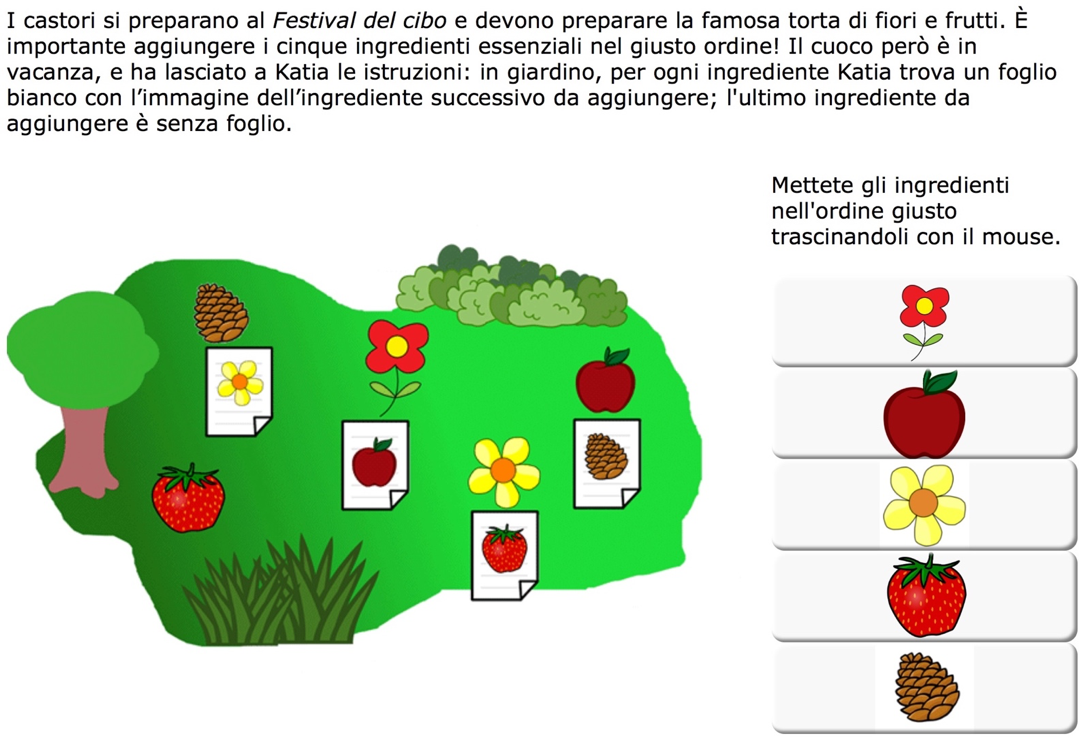
\includegraphics[height=10.0cm]{2016-HU-02Testo.png}
	\caption{La ricetta segreta (2016-HU-02)}\label{fig:1}
\end{figure}
Questo quesito era presente nella gara svolta nel novembre 2016, all'interno della categoria KiloBebras.

La lista degli ingredienti è un esempio della struttura dati chiamata lista. Il foglio che indica l'ingrediente successivo costituisce il puntatore all'elemento successivo della lista. Per accedere alla lista occorre avere il puntatore al primo elemento della lista.
%
%
%
\\
\begin{figure}[H]
	\centering
	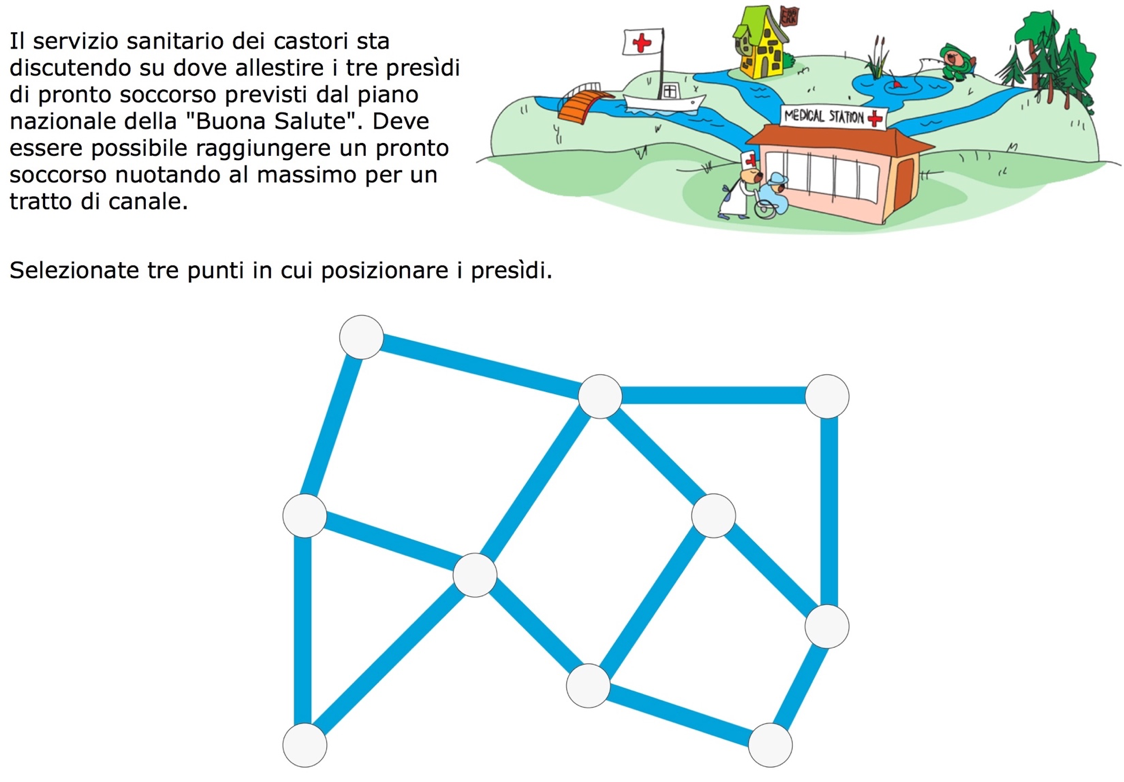
\includegraphics[height=11.0cm]{2016-CH-03Testo.png}
	\caption{Pronto soccorso (2016-CH-03)}\label{fig:2}
\end{figure}
Questo quesito era presente nella gara svolta nel novembre 2016, all'interno della categoria MegaBebras, GigaBebras e TeraBebras.

La rete di canali raffigurata può essere rappresentata da un grafo, in cui i tratti di canale sono gli archi (non orientati, cioè percorribili in entrambi i sensi) e i punti dove essi si incontrano sono i nodi. Il quesito proposto è un esemplare del problema dell’insieme dominante nella versione in cui si tratta di decidere se un insieme dominante esiste. 

\section{Classificazione quesiti}
Dalla nascita del Bebras, nel 2004, fino ad oggi sono stati redatti un numero ingente di quesiti. All'interno della comunità è quindi nata l'esigenza di classificarli per poter creare quesiti più eterogenei ed equilibrati rispetto ai concetti trattati.

La prima classificazione dei quesiti all'interno della comunità Bebras che è stata proposta nel 2008 da Dagiene e Futschek\cite{DagieneISEEP2008}, consiste nelle seguenti categorie:
\begin{itemize}
\item \textbf{comprensione dei dati}
attraverso la rappresentazione simbolica, numerica e visiva, la codifica, la crittografia

\item \textbf{ragionamento algoritmico},
compresi gli aspetti di programmazione

\item \textbf{uso di sistemi informatici}
come motori di ricerca, email, fogli elettronici; principi generali senza riferimento ad uno specifico sistema

\item \textbf{strutture, patterns e ottimizzazione combinatoria}
come i grafi

\item \textbf{puzzles}
come giochi logici

\item \textbf{l'Informatica e la società}
includendo argomenti sociali, etici e culturali riguardanti la disciplina informatica
\end{itemize}

Tale classificazione, nonostante sia stata utilizzata per molto tempo, è risultata troppo generica per essere applicata alla grande varietà di quesiti Bebras, inoltre alcune categorie spesso non vengono utilizzate perché molto legate ad aspetti non attinenti agli attuali quesiti Bebras.
Successivamente nel 2009 è stata proposta da Kalas e Tomcsanyiova\cite{KalasIFIP2009} un'altra tecnica di classificazione basata sugli argomenti informatici trattati, ogni quesito poteva essere inserito in una o due categorie:
\begin{itemize}
	\item \textbf{alfabetizzazione digitale}: conoscenze di base, concetti di informatica, uso del computer, questioni etiche e legali, sicurezza, storia dell'informatica
	\item \textbf{programmazione}: descrizione formale di una soluzione, di un processo o di un comportamento; comprensione, analisi, interpretazione di una descrizione; algoritmi e pensiero algoritmico
	\item \textbf{risoluzione di un problema}: ragionamento logico e argomentazione; puzzles, enigmi e problemi; strategie per la soluzione dei problemi
	\item \textbf{gestione dei dati}: rappresentazioni di dati, codifiche, patterns, strutture dati
\end{itemize}

Più recentemente, nel 2015, è stata proposta da Pohl e Westmeyer \cite{PohlLNCS2015} una classificazione gerarchica basata sull'idea principale di Schwill \cite{SchwillEATCS1994}.
I nodi-padre di tale gerarchia proposta sono:
\begin{itemize}
	\item \textbf{algoritmizzazione}: concetti di programmazione, valutazione della complessità, verifica della correttezza, processi concorrenti, ... 
	\item \textbf{organizzazione strutturale}: modularizzazione, gerarchizzazione, ortogonalizzazione
	\item \textbf{formalizzazione}: sintassi e semantica
	\item \textbf{sistemi informatici}: applicazioni informatiche
\end{itemize}

\'{E} stata proposta tale struttura gerarchica per permettere una classificazione a grana fine e su livelli di dettaglio diversi.

In seguito è stata presentata una classificazione ortogonale \cite{DagieneKEYCIT2015} a partire dalla Tassonomia di Bloom.
Quest'ultima è uno dei modi di formalizzare le fasi di acquisizione di informazioni attraverso la classificazione degli scopi educativi. In particolare i settori della tassonomia di Bloom fanno riferimento ai vari obiettivi che gli educatori dovrebbero definire per i loro studenti. Tali obiettivi sono divisi in tre domin\^{i}: cognitivo, affettivo e psicomotore. All'interno di tali domin\^{i}, il passaggio al livello successivo è pregiudicato dall'acquisizione delle conoscenze e abilità che precedono.
Questa tassonomia, insieme alla classificazione di Kalas precedentemente esposta \cite{KalasIFIP2009}, genera la seguente classificazione ortogonale:
\begin{itemize}
	\item Ricordare fatti generali, concetti di base
	\item Comprensione semplice di un dato linguaggio, di comandi e del loro significato
	\item Comprensione complessa della descrizione di processi, di regole e di metodi
	\item Applicare delle regole generative o metodi ad uno stato iniziale o input
	\item Interpretare date istruzioni o programmi
	\item Analizzare condizioni o processi
	\item Analizzare le corrispondenze di più descrizioni con più comportamenti
	\item Analizzare diverse situazioni o soluzioni in base a dati criteri
	\item Dedurre un possibile risultato, uno stato finale o un prodotto finale
	\item Mettere insieme informazioni
\end{itemize}

Nel 2017 vengono proposte due nuove classificazioni basate sulla definizione operazionale del pensiero computazionale sviluppata dall'ISTE (International Society for Technology in Education) e dal CSTA (Computer Science Teachers Association) \cite{flayerCT}.

La prima classificazione \cite{DagieneINFORMATICA2017} è composta da due dimensioni, nello specifico la dimensione delle abilità del pensiero computazionale e quella rappresentante i concetti informatici.
\newpage
La prima dimensione è così costituita:
\begin{itemize}
	\item \textbf{astrazione}: rimuovere dettagli non necessari, riconoscere elementi chiave, scegliere la rappresentazione di un sistema
	\item \textbf{pensiero algoritmico}: ragionare in termini di sequenze e di regole, eseguire un algoritmo, creare un algoritmo
	\item \textbf{scomposizione}: decomporre in sottoproblemi, ragionare su un problema in termini di sottoproblemi
	\item \textbf{valutazione}: trovare la soluzione migliore, prendere buone decisioni riguardo l'uso di risorse a disposizione
	\item \textbf{generalizzazione}: identificare patterns, risolvere nuovi problemi sulla base di problemi già risolti, utilizzare soluzioni generali in una specifica circostanza
\end{itemize}

La seconda dimensione è così definita:
\begin{itemize}
	\item \textbf{algoritmi e programmazione}: algoritmi, ricerca binaria, algebra booleana, etc.
	\item \textbf{dati, strutture dati, rappresentazione dati}: array, database, grafi, liste, code, etc.
	\item \textbf{processi e hardware}: deadlock, processamento di immagini, macchina di Turin, etc.
	\item \textbf{comunicazione e rete}: client/server, crittografia, protocolli, sicurezza, etc.
	\item \textbf{interazione, sistemi e società}: uso del computer, etica, virus, etc.
\end{itemize}

Si ottiene, quindi, una matrice bidimensionale in cui ogni quesito può essere posto in una sola categoria di concetti informatici ma in più categorie rappresentanti le abilità del pensiero computazionale.
\begin{figure}[H]
	\centering
	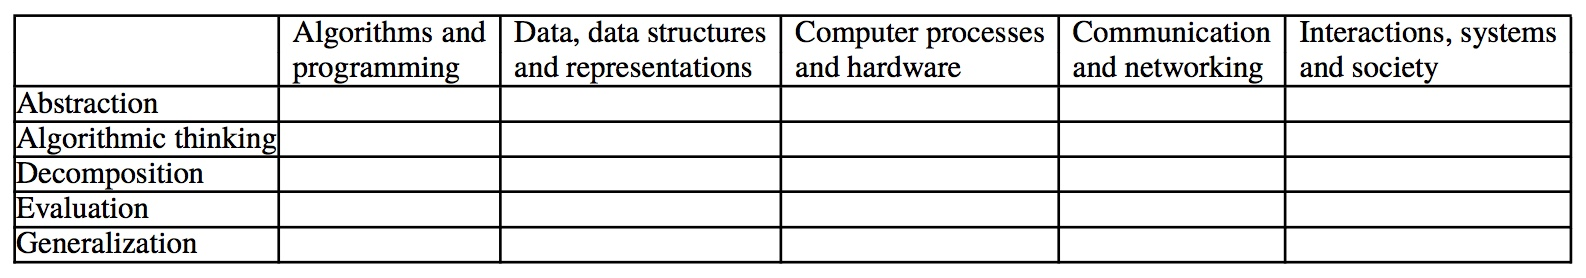
\includegraphics[height=2.7cm]{two-dimensional_classification.jpeg}
	\caption{Classificazione a due dimensioni}\label{fig:3}
\end{figure}

Infine la seconda classificazione \cite{LonatiITICSE2017}, che si basa anch'essa sulla definizione di pensiero computazionale definito dall'ISTE e dal CSTA, ha come obiettivo principale evidenziare il potenziale didattico dei quesiti Bebras.
Si vuole rendere comprensibile la classificazione anche a docenti senza una formazione informatica, inoltre tale approccio evidenzia le abilità cognitive coinvolte in un quesito e quindi il suo potenziale educativo.

Questa classificazione è così composta:
\begin{itemize}
	\item \textbf{Organizzazione logica dei dati}: organizzazione dei dati secondo certi criteri fissati (come ad esempio in una tabella), uso di strutture per rendere i dati più facili da elaborare, organizzare i dati in modo che godano di proprietà interessanti come nel caso della crittografia o della compressione dei dati.
	\item \textbf{Analisi logica dei dati}: “problemi logici” che si basano sul ragionamento logico-deduttivo e che chiedono di trarre conclusioni relative ai dati presentati nel quesito, quesiti che richiedono di osservare attentamente gli oggetti coinvolti (es: per riconoscere elementi simili o ricorrenti) o di procedere in maniera sistematica per stabilire se i dati del problema soddisfano o meno certe proprietà.
	\item \textbf{Rappresentazione digitale dell'informazione}: rappresentazione simbolica dei dati, rappresentazione visuale tramite diagrammi come istogrammi o grafici, strutture di dati che consentono di rappresentare proprietà interessanti (ad esempio: relazioni binarie o gerarchiche tra oggetti).
	\item \textbf{Pensiero algoritmico}: uso di metodi sistematici o procedure passo-passo, andando oltre la pura idea intuitiva su come risolvere il problema, ad esempio tramite la scomposizione del problema in sotto-problemi; la combinazione di operazioni elementari per svolgere un compito più complesso; l’uso di procedure formali (da eseguire o di cui calcolare/prevedere il risultato); l’applicazione di regole di transizione ad un sistema che si trova in un certo stato di partenza, ecc.
	\item \textbf{Identificare strategie risolutive}: ricerca di strategie algoritmiche non scontate per risolvere un problema.
	\item \textbf{Analizzare soluzioni algoritmiche}: quesiti che riguardano le caratteristiche generali di un algoritmo o di un metodo risolutivo presentato nel quesito, quali la correttezza del metodo o la sua praticabilità, quesiti che si ispirano a problemi di ottimizzazione, in cui si cerca la soluzione “migliore” tra tutte le soluzioni accettabili.
	\item \textbf{Implementare soluzioni algoritmiche}: problemi di programmazione o “coding”, si concentrano sull’implementazione di algoritmi attraverso l’uso di una sintassi formale definita nel quesito.
\end{itemize}

%
\section{Il Bebras in Italia}
Ogni delegazione della comunità internazionale del Bebras, come detto nella sezione 1, cura lo svolgimento della gara in locale.
In Italia il Bebras si svolge in un tempo massimo di 45 minuti attraverso una piattaforma su computer, nella settimana fissata dalla comunità internazionale, solitamente nel mese di novembre. Tali gare vengono proposte agli studenti dividendoli in gruppi da quattro componenti, infatti lavorare in squadra è un aspetto fondamentale.
Ogni gara è composta da 15 quesiti, diversamente dalle altre delegazioni Bebras, in Italia vengono proposti pochi quesiti con domande a risposta multipla. I quesiti scelti per l'edizione italiana sono in maggior parte domande interattive o domande che richiedono una complessa combinazione di risposte. Viene considerato anche un punteggio parziale per alcuni quesiti e non ci sono penalità per eventuali risposte errate.

In ogni categoria i quesiti sono divisi in tre livelli di difficoltà, ognuno dei quali corrisponde all'incremento di punti che possono essere accumulati.
Alcuni quesiti sono ripetuti in più categorie ma con un diverso livello di difficoltà e quindi una differente assegnazione di punteggio. In particolare l'intenzione degli organizzatori è che ogni categoria possa avere una coppia di quesiti che siano accessibili a tutti e una coppia in cui è richiesto un maggiore ragionamento. 

I partecipanti sono divisi in categorie in relazione alla classe frequentata:
\begin{itemize}
	\item \textbf{KiloBebras}: alunni delle Scuole Primarie [8-10 anni circa]
	\item \textbf{MegaBebras}: alunni delle classi prima e seconda delle Scuole Secondarie di primo grado [10-12 anni circa]
	\item \textbf{GigaBebras}: alunni delle classi terze delle Scuole Secondarie di primo grado [12-13 anni circa]
	\item \textbf{TeraBebras}: alunni del biennio delle Scuole Secondarie di secondo grado [13-15 anni circa]
	\item \textbf{PetaBebras}: alunni del triennio delle Scuole Secondarie di secondo grado [15-18 anni circa]
\end{itemize}

Ogni docente è invitato a discutere la correzione dei quesiti in classe  come occasione per approfondire o chiarire gli argomenti trattati. Spesso i docenti stessi richiedono la presenza di alcuni rappresentanti della delegazione italiana Bebras per poter svolgere la correzione insieme. Quest'ultima diventa un'occasione non solo per i partecipanti ma anche per gli stessi organizzatori che possono rilevare e osservare alcune criticità dell'edizione svolta e successivamente riflettere su eventuali correzioni per gli anni successivi.
A tal proposito la delegazione italiana ha svolto delle interviste \cite{LonatiKoli2017} in nove classi (circa 180 studenti) che hanno partecipato al Bebras nel 2016 con l'obiettivo di raccogliere commenti e individuare le difficoltà incontrate nella gara. 
A partire dalle osservazioni rilevate, sono stati modificati alcuni quesiti e riproposti a nuove classi per verificarne la correzione effettuata.

% [è necessario espandere maggiormente questa parte???]


%			CAPITOLO 2: Indicazioni nazionali e Bebras
\chapter{Indicazioni nazionali e Bebras}
\label{cap2}

%
%
%			CAPITOLO 3: CT e Bebras
\chapter{CT e Bebras}



\label{cap3}
%
%

%
%			BIBLIOGRAFIA
%
\begin{thebibliography}{00}
%
\bibitem{BellettiniITICSE2015}
C. Bellettini, V. Lonati, D. Malchiodi, M. Monga, A. Morpurgo, M. Torelli, 
"How challenging are Bebras tasks? An IRT analysis based on the performance of Italian students", 
Proceedings of the 2015 ACM Conference on Innovation and Technology in Computer Science Education (ITiCSE 2015), 
pp. 27-32, 
Lithuania, 
July, 6-8, 
2015.
%
\bibitem{DagieneIFIP2010}
V. Dagiene, G. Futschek, 
"Introducing Informatics Concepts through a Contest", 
IFIP working conference: New developments in ICT and education, 
Amiens: Universite de Picardie Jules Verne, 
2010.
%
\bibitem{LonatiITICSE2017}
V. Lonati, D. Malchiodi, M. Monga, A. Morpurgo, 
"Bebras as a teaching resource: classifying the tasks corpus using computational thinking skills", 
Proceedings of the 22nd annual conference on innovation and technology in computer science education (ITiCSE 2017) 
Bologna, Italy, 
2017.
%
\bibitem{DagieneISEEP2008}
V. Dagiene, G. Futschek, 
"Bebras international contest on informatics and computer literacy: Criteria for good tasks", 
ISSEP 2008, 
LNCS, vol. 5090, 
pp. 19–30, 
2008.
%
\bibitem{DagieneINFORMATICA2017}
V. Dagiene, S. Sentence, G. Stupuriene, 
"Developing a Two-Dimensional Categorization System for Educational Tasks in Informatics", 
Informatica, vol. 28, no.1, 
pp.23-44, 
2017.
%
\bibitem{flayerCT}
International Society for Technology in Education \& Computer Science Teachers Association, 
"Operational definition of computational thinking for K-12 education."
\url{https://csta.acm.org/Curriculum/sub/ CurrFiles/CompThinkingFlyer.pdf}, 
2011.
%
\bibitem{DagieneISSEP2016}
V. Dagiene, S. Sentance, 
"It’s computational thinking! bebras tasks in the curriculum", 
ISSEP 2016, 
LNCS, vol. 9973, 
pp. 28–39, 
2016.
%
\bibitem{indicazioniNazionali}
Indicazioni nazionali riguardanti gli obiettivi specifici di apprendimento concernenti le attività e gli insegnamenti compresi nei piani degli studi previsti per i percorsi liceali di cui all'art. 10, comma 3, del DPR 15/3/2010, n. 89, in relazione all'art. 2, commi 1 e 3, del medesimo regolamento, 2010.
%
\bibitem{DagieneKEYCIT2015}
V. Dagiene, G. Stupuriene, 
"Informatics education based on solving attractive tasks through a contest", 
KEYCIT 2014 - Key Competencies in Informatics and ICT, 
pp. 97 – 115, 
2015.
%
\bibitem{HabermanACM2011}
B. Haberman, A. Cohen, V. Dagiene, 
"The beaver contest: attracting youngsters to study computing", 
Proceedings of the 16th annual joint conference on Innovation and technology in computer science education, ACM, 
p. 378, 
2011.
%
\bibitem{LonatiISSEP2017}
V. Lonati, M. Monga, A. Morpurgo, D. Malchiodi, A. Calcagni, 
"Promoting computational thinking skills: would you use this Bebras task?", 
Proceedings of the international conference on informatics in schools: situation, evolution and perspectives (ISSEP2017) (in stampa) 
Helsinki, Finland, 
2017.
%
\bibitem{KalasIFIP2009}
I. Kalaš, M. Tomcsányiová, 
"Students’ Attitude to Programming in Modern Informatics", 
IFIP World Conference on Computers in Education, 
Bento Goncalves, Brazil, 
2009.
%
\bibitem{PohlLNCS2015}
W. Pohl, J. Westmeyer, 
"Content categories for informatics tasks", 
LNCS, vol.9378, 
pp. 61-62,
2015. 
%
\bibitem{SchwillEATCS1994}
A. Schwill, 
"Fundamental ideas of computer science", 
EATCS-Bulletin, vol. 53, 
pp. 274– 295, 
1994.
%
\bibitem{LonatiKoli2017}
V. Lonati, D. Malchiodi, M. Monga, A. Morpurgo, 
"How presentation affects the difficulty of computational thinking tasks: an IRT analysis.", 
Proceedings of the 17th koli calling international conference on computing education research (in stampa),
Koli, Finland, 
2017.
%
\end{thebibliography}
% 
%			RINGRAZIAMENTI
%
\prefacesection{Ringraziamenti}
asdjhgftry.
\end{document}


 
